\section{关键技术}

\subsection{存储}

图数据库的存储技术是其核心组成之一, 直接影响到数据库的性能和扩展性。图数据库存储方式包括原生图存储和非原生图存储。

\subsubsection{原生图存储}

原生图存储是专门为图数据而设计的存储方式, 能够自然地存储节点、边及其属性。由于原生图存储以图为基本单元, 存储结构和图的物理结构保持一致, 因此可以直接、高效地进行节点间的遍历操作。原生图存储通常采用\textbf{邻接列表或邻接矩阵}作为其底层数据结构。
邻接列表是一种常见的图数据存储方式, 如\cref{fig:adjacency-list}所示, 对于每个节点, 存储一个列表以记录其相邻节点。邻接列表的优势在于存储空间效率高, 特别适用于稀疏图, 因为只需存储存在的边。其劣势在于, 当需要快速查找两个节点之间的关系时, 可能需要遍历整个邻接列表。\begin{figure}[H]
	\centering
	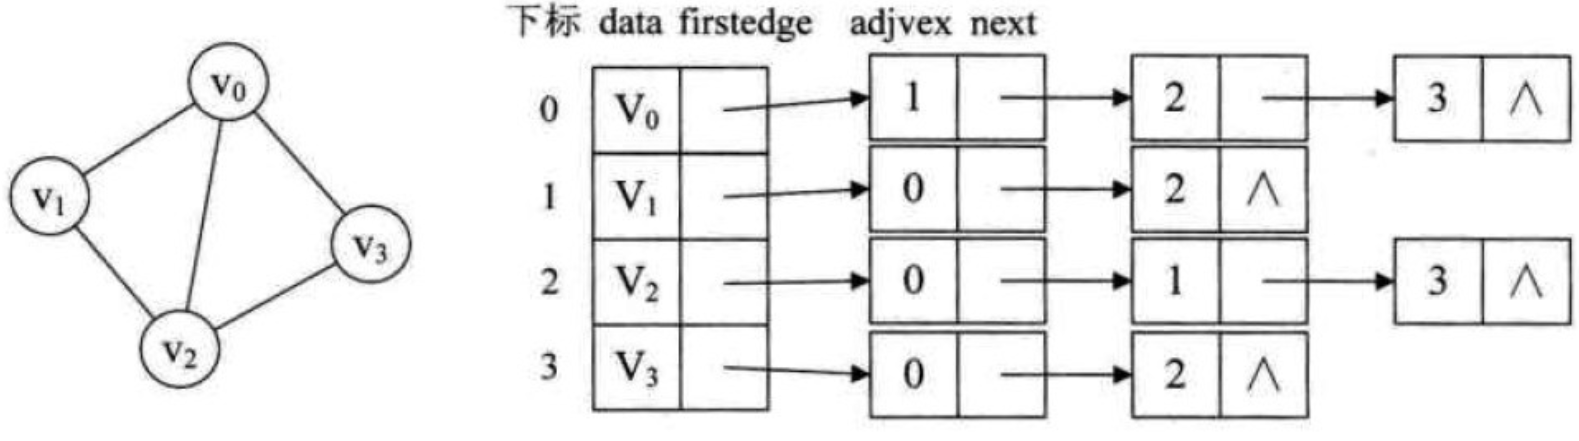
\includegraphics[width=1\textwidth]{images/11.png}
	\caption{邻接列表}
	\label{fig:adjacency-list}
\end{figure}

Neo4j是最具代表性的原生图数据库, 其存储引擎专门针对图遍历进行了优化, 使得复杂关系查询的性能得以保障。如\cref{fig:neo4j}所示, Neo4j的存储方式结合了指针和嵌入式存储, 使得在遍历节点和边时可以实现低延迟的高效访问。\begin{figure}[H]
	\centering
	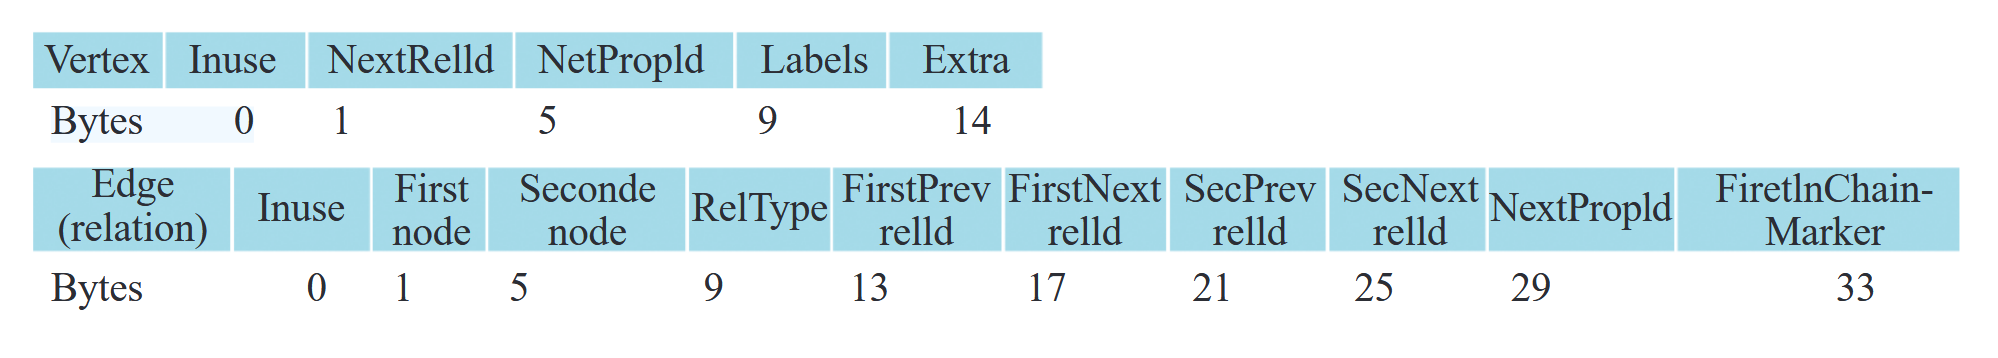
\includegraphics[width=1\textwidth]{images/4.png}
	\caption{Neo4j的存储结构}
	\label{fig:neo4j}
\end{figure}

\cref{tab:neo4j-vertex}展示了Neo4j中节点的存储结构, 其中包括节点的有效性、关联关系的指针、标签等信息。\begin{table}[H]
	\centering
	\caption{Neo4j的vertex存储结构}
	\begin{tabular}{|c|c|c|}
		\hline
		顶点字段       & 字节位置 & 说明              \\
		\hline
		inUse      & 0    & 是否有效            \\
		nextRelId   & 1-4  & 关联到该节点的第一个关系的id \\
		nextPropId & 5-8  & 关联到该节点的第一个属性的id \\
		labels     & 9-13 & 指向标签的指针         \\
		extra      & 14   & 存储内部标志信息        \\
		\hline
	\end{tabular}
	\label{tab:neo4j-vertex}
\end{table}
Neo4j通过其独特的存储结构实现了高效的图数据处理能力。在节点存储方面, Neo4j采用了紧凑的定长14字节结构, 保存在文件neostore.nodestore.db。其中包含了关键的nextRelId字段用于存储第一个关联关系的ID, 为快速图遍历提供了入口点。同时, nextPropId字段直接链接到节点的属性存储, 实现了属性的快速访问, 而labels字段则通过直接指针定位标签信息, 避免了额外的查找开销。这种紧凑的存储结构不仅节省了存储空间, 更重要的是提高了缓存效率。此外, 由于每个结点的存储结构是固定长度的, 因此可以通过简单的偏移计算来快速定位节点, 从而实现高效的图遍历操作。

\cref{tab:neo4j-edge}展示了Neo4j中边的存储结构, 包括边的有效性、起始节点和终止节点的id、边的类型等信息。通过这种存储方式, Neo4j能够高效地存储和查询图数据, 并支持复杂的图遍历操作。\begin{table}[H]
	\centering
	\caption{Neo4j的Edge存储结构}
	\begin{tabular}{|c|c|c|}
		\hline
		顶点字段              & 字节位置  & 说明             \\
		\hline
		inUse             & 0     & 是否有效           \\
		firstNode         & 1-4   & 关系的起始节点id      \\
		secondNode        & 5-8   & 关系的终止节点id      \\
		relationshipType           & 9-12  & 关系的类型          \\
		firstPrevRelId     & 13-16 & 指向起始顶点上前一个边的指针 \\
		firstNextRelId     & 17-20 & 指向起始顶点上后一个边的指针 \\
		secondPrevRelId      & 21-24 & 指向终止顶点上前一个边的指针 \\
		secondNextRelId      & 25-28 & 指向终止顶点上后一个边的指针 \\
		nextPropId         & 29-32 & 与边关联的下一个属性的id    \\
		firstInChainMaker & 33-34 & 是否为关系链的第一条边    \\
		\hline
	\end{tabular}
	\label{tab:neo4j-edge}
\end{table}
在边的存储结构设计上, Neo4j采用了更为复杂的机制。关系是存放在 \\ neostore.relationship.store.db 中, 通过firstPrevRelId、firstNextRelId等字段构建的双向链表结构, 使得系统能够高效地在相关节点间进行双向遍历。边存储直接包含了起始和终止节点的ID, 避免了间接寻址带来的性能损耗。同时, relationshipType字段的设计支持关系类型的快速过滤, 而firstInChainMaker的标记则有助于关系链的快速识别和处理。这种存储结构使得图的遍历操作能够保持较低的延迟。此外, 由于关系的存储结构是固定长度的,因此可以通过简单的偏移计算来快速定位关系,从而实现高效的图遍历操作。


属性记录的物理存储放置在neosore.propertystore.db文件中。与节点和关系的存储记录一样, 属性的存储记录也是固定长度。每个属性记录包含属性块和属性链中下一个属性结点的ID。属性链是单向链表, 而关系链是双向链表。一个属性记录中可以包含任何 Java 虚拟机 (JVM) 支持的基本数据类型、字符串、基于基本类型的数组以及属性索引文件 (neostore.propertystore.db.index) 。属性索引文件主要用于存储属性的名称, 属性索引的值部分存储的是指向动态内存的记录或者内联值, 短字符串和短数组会直接内联在属性存储记录中。当长度超过属性记录中的 propBlock 长度限制之后, 会单独存储在其他的动态存储文件中。


\subsubsection{原生图遍历}

\Cref{fig:neo4j-case} 就是节点、关系、属性在 Neo4j 中的物理表现方式。图中直接看起来可能不是那么直观,可以想象关系是属于两个节点的, 但是一个关系也不应该在记录中出现两次, 这样会造成内存的浪费。因此两个双向链表之间会有指针, 一个是起始节点可见的列表关系, 另一个是结束节点可见的列表关系。每一个列表都是双向链表, 因此我们可以在任何一个方向上进行快速遍历和高效地插入和删除。
\begin{figure}[H]
	\centering
	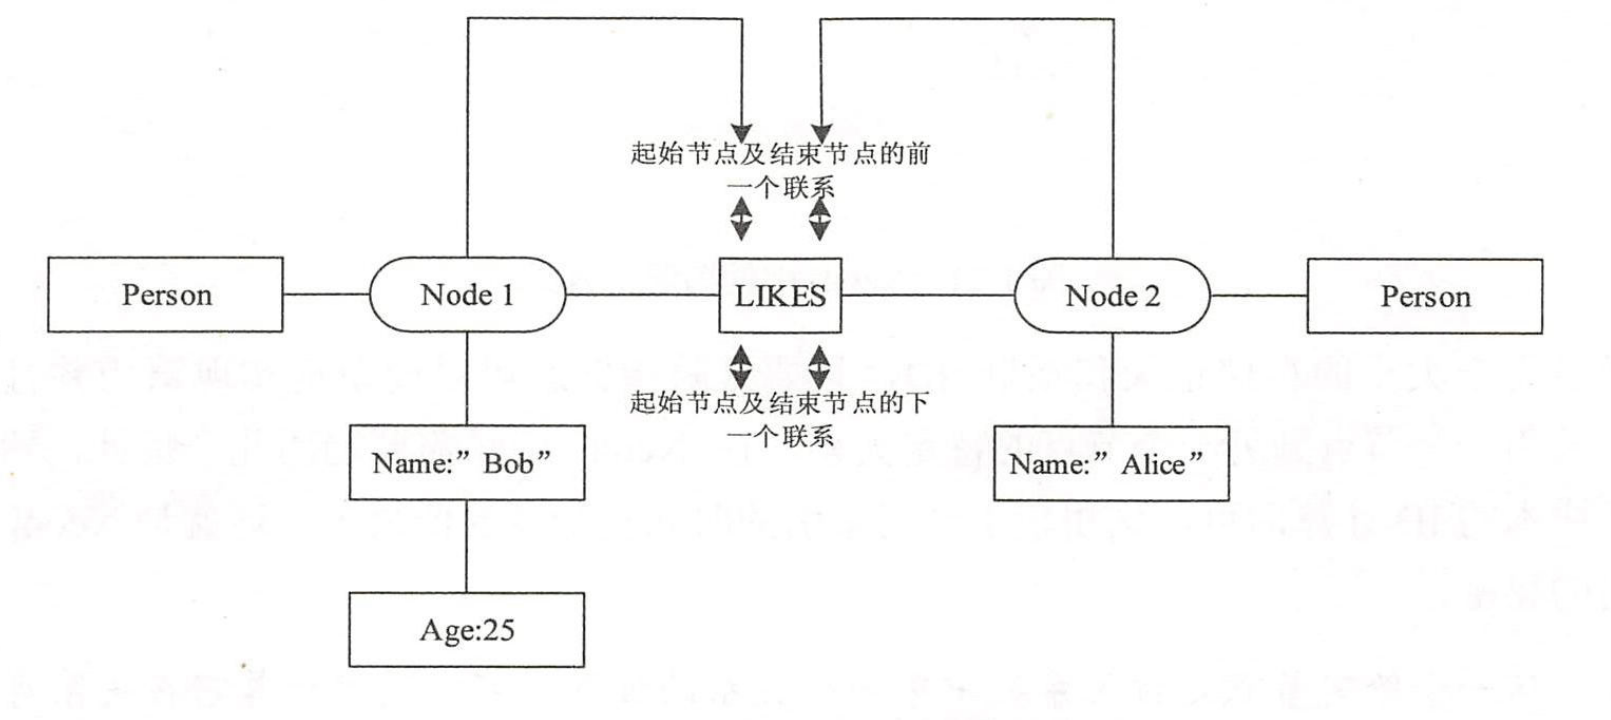
\includegraphics[width=1\textwidth]{images/18.png}
	\caption{Neo4j的存储结构例子}
	\label{fig:neo4j-case}
\end{figure}

下面通过一个例子来讲解 Neo4j 遍历关系和节点的详细过程。假如在 Neo4j 中存储了A、B、C、D、E共5个节点和R1、R2、R3、R4、R5、R6、R7共7个关系, 它们之间的关系如\cref{fig:case2}所示。
\begin{figure}[!t]
	\centering
	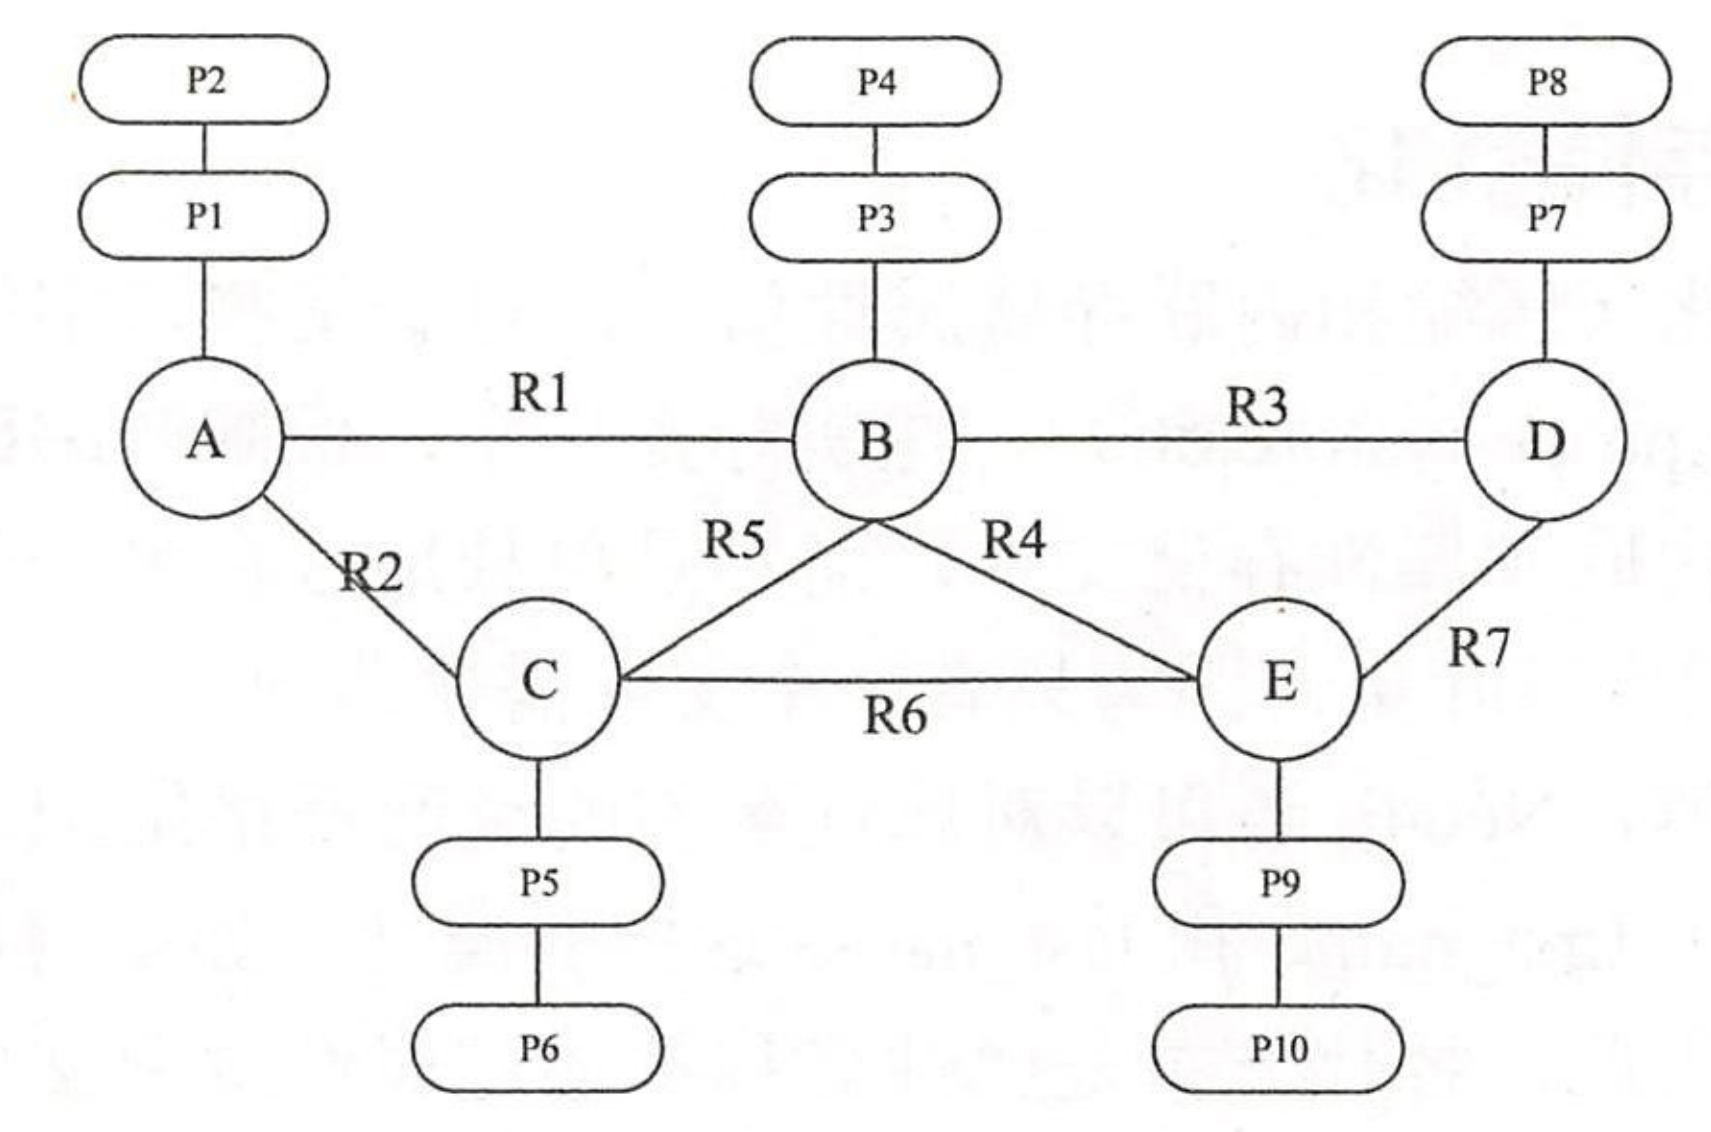
\includegraphics[width=0.8\textwidth]{images/19.png}
	\caption{Neo4j的存储结构例子: 抽象图结构}
	\label{fig:neo4j-case2}
\end{figure}
假如要遍历图中节点B的所有关系, 只需要向NODEB-NEXT方向遍历, 直到指向NULL为止, 可以从\cref{fig:traverse}中看出节点B的所有关系为R1、R3、R4、R5。
\begin{figure}[H]
	\centering
	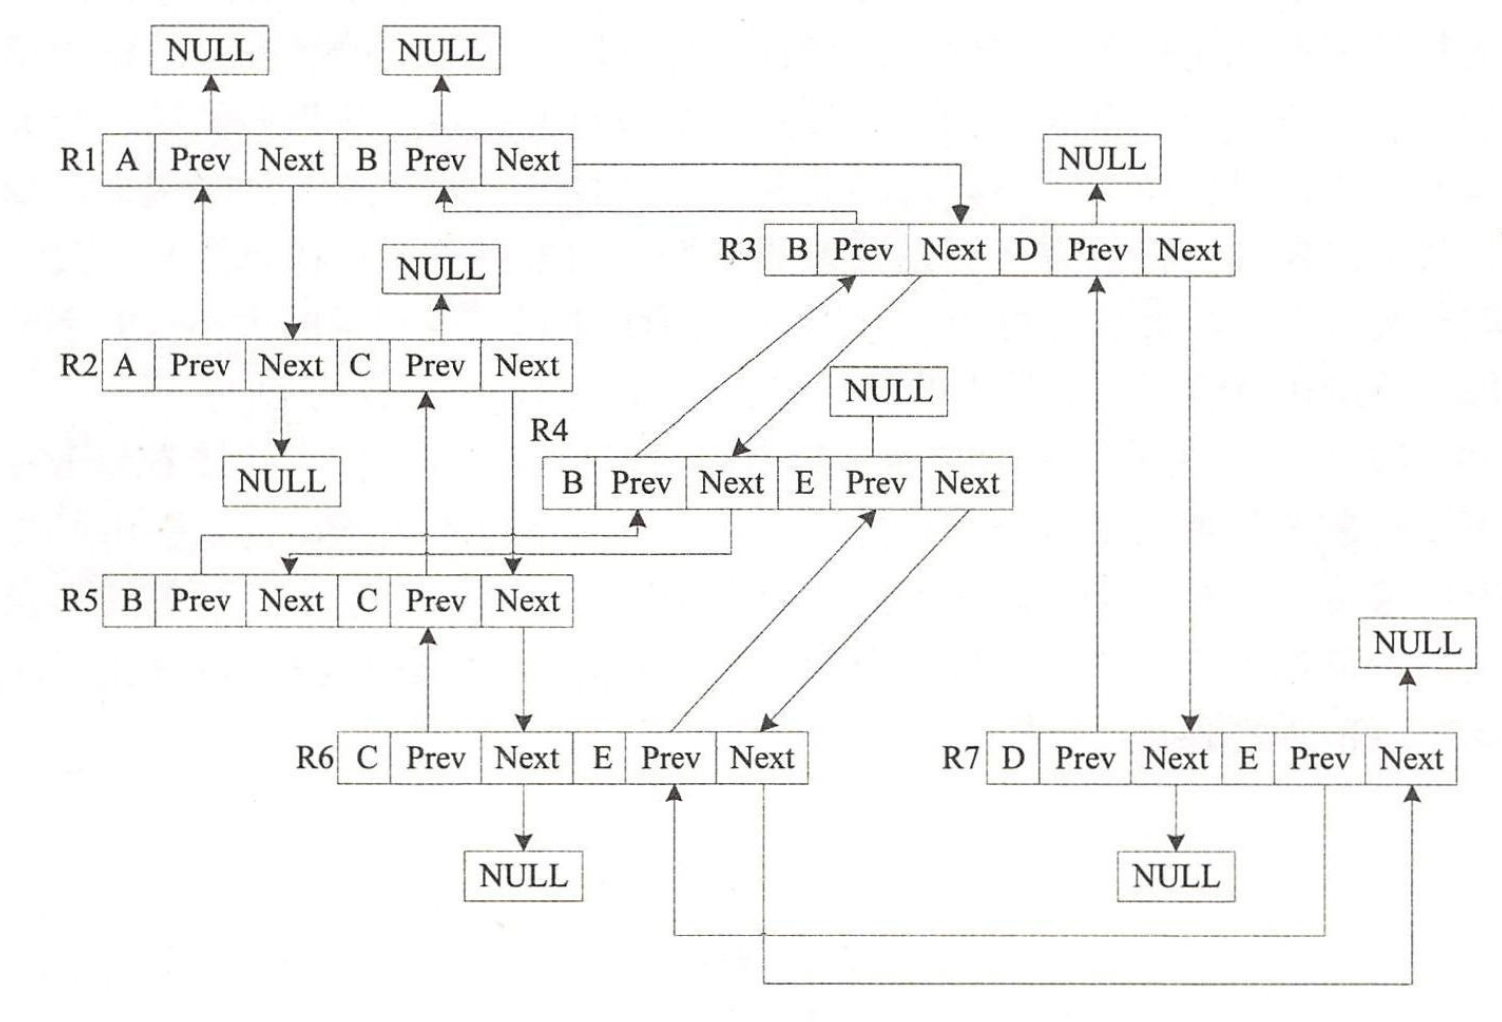
\includegraphics[width=1\textwidth]{images/20.png}
	\caption{Neo4j的存储结构例子: 边的存储结构}
	\label{fig:neo4j-traverse }
\end{figure}
通过固定大小的存储记录和指针ID, 只要跟随指针就可以简单地实现遍历并且高速执行。要遍历一个节点到另一个节点的特定关系, 在Neo4j中只需要遍历几个指针, 然后执行一些低成本的ID计算即可, 这相较于全局索引的时间复杂度要低很多。




\subsubsection{非原生图存储}

非原生图存储是基于已有的通用数据库(如键值存储)来支持图数据存储的方案。如\cref{fig:janusgraph-vertex}所示, 这种存储方式通过将节点和边映射到表或键值对中进行存储, 常用的数据结构包括关系表和键值对映射。\begin{figure}[H]
	\centering
	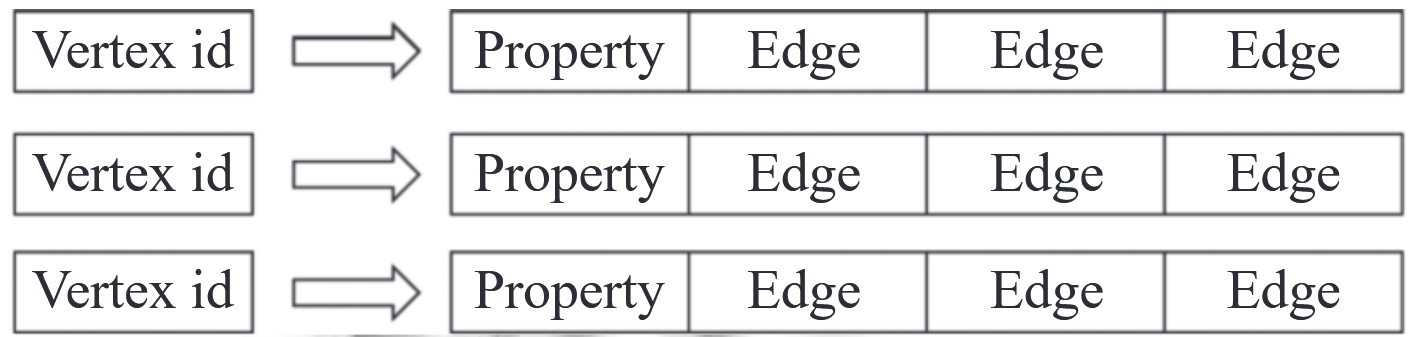
\includegraphics[width=\textwidth]{images/6.png}
	\caption{非原生图存储}
	\label{fig:non-native}
\end{figure}
\cref{fig:janusgraph-vertex}展示了JanusGraph的Vertex存储结构, 其中vertex id共包含一个字节, 8位, 64 bit, 分为3个部分: partition id、count、ID padding。前5位为partition id, partition 是 JanusGraph 抽象出的概念, 通过其数量计算可以最终使数据均匀分配到多台机器中。中间的count是流水号, 最高位固定为 0, 其剩余位数足以生成2的55次幂个id, 满足节点数量生成。最后几位bit是ID padding, 表示Vertex的类型,具体位数长度会随不同类型有所修改, 常用情况值为“000”。\begin{figure}[H]
	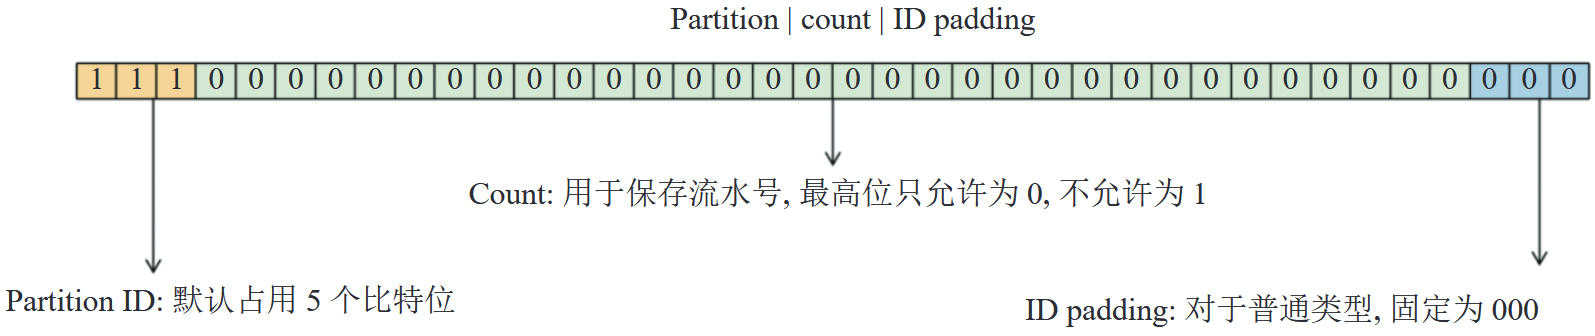
\includegraphics[width=1\textwidth]{images/12.png}
	\caption{JanusGraph的Vertex存储结构}
	\label{fig:janusgraph-vertex}
\end{figure}
\cref{fig:janusgraph-edge}给出了Edge和Property的逻辑结构, 均分别由column和value两部分组成。在Edge的column中,包含了label id、direction、sort key、adjacent vertex id和edge id。其中, label id是边类型代表的 id。Direction是图的方向, 用0和1来分别代表出和入。Sort key可以指定多个边的属性。Adjacent vertex id是目标节点 id,实际存储的是目标节点id和源节点id的差值。Edge id则是边的全局唯一id。Edge的value由signature key和other property组成, 前者用于提升edge的属性的检索速度, 后者则是存储边的其他属性。Property的column包含key id和property id, 前者用于存储属性label对应的id值, 后者则是指定属性的唯一id。Value中只有property value用于保存属性值。
\begin{figure}[H]
	\centering
	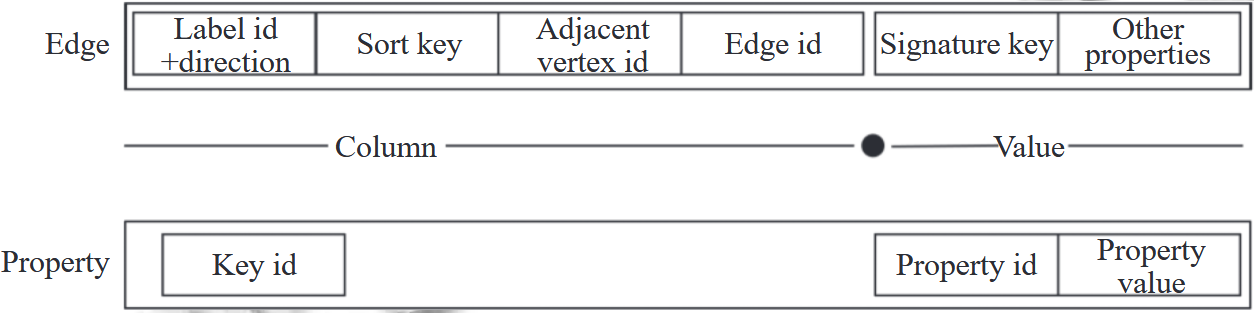
\includegraphics[width=0.8\textwidth]{images/13.png}
	\caption{JanusGraph的Edge存储结构}
	\label{fig:janusgraph-edge}
\end{figure}

非原生图存储的优点在于扩展性强, 可以利用已有数据库系统的可靠性和分布式能力, 适合超大规模数据存储的需求;但由于其底层并非针对图结构优化, 因此在图遍历和复杂查询方面性能有限, 尤其在深度查询和多跳查询的情况下表现不如原生存储高效。

\subsection{查询}

图数据库的查询功能是其核心优势之一, 通过查询语言和算法的结合, 使得用户能够高效地从图中获取信息。图数据库的查询主要包括命令式查询语言、声明式查询语言以及支持的图遍历和分析算法。
\subsubsection*{命令式查询语言}

命令式查询语言要求用户明确指定如何执行查询操作, 包括每一步遍历和过滤的详细指令。Apache TinkerPop的Gremlin是一个典型的命令式查询语言, 其查询风格类似于编程, 用户需要指定每一步的节点或边的操作。Gremlin适合灵活、复杂的查询需求,但对用户的编程能力要求较高。通过命令式查询, 用户可以对图数据进行逐步遍历, 从而实现复杂的多跳查询和条件筛选。
例如, 假设我们有一个社交网络图数据库, 其中节点代表用户, 边代表好友关系。要查找某个用户的好友的好友, 可以使用以下Gremlin查询:

\tbox{g.V () .has ('name','Alice') .out ('knows') .out ('knows') .values ('name') }

这段代码的含义是: 找到名称为“Alice”的节点, 然后遍历其所有的“knows”关系, 接着再遍历这些好友节点的“knows”关系, 最后返回这些好友的好友的名称。

\subsubsection*{声明式查询语言}

声明式查询语言则让用户关注“要查询什么”而不是“如何查询”。Neo4j的Cypher语言就是一种典型的声明式查询语言。Cypher通过类似SQL的语法, 用户可以方便地描述想要查询的图结构和条件, 而无需指定遍历的细节。Cypher语法简洁, 类似于SQL, 因此也易于学习, 对于常见的查询需求如模式匹配和路径查找非常高效。例如, 在社交网络图数据库中, 假设我们要查找名称为“Alice”的用户的好友, 可以使用以下简单的一行Cypher查询语句:

\tbox{MATCH  (a:Person {name: 'Alice'}) -[  ]-> (friend)  RETURN friend.name}

声明式查询语言的优势在于易用性强, 用户可以快速上手并实现复杂的查询, 而无需了解底层遍历细节。这对于大多数应用场景是非常友好的, 尤其在社交网络和推荐系统中, Cypher被广泛应用。

\subsubsection*{Cypher、Gremlin、GSQL介绍与对比}
Cypher、Gremlin和GSQL是图数据库领域最常见的三种查询语言, 各有优缺点。
\begin{table}[htbp]
	\centering
	\caption{三种图查询语言对比}
	\begin{tabularx}{\textwidth}{|X|X|X|X|}
		\hline
		查询语言  & Cypher                       & Gremlin              & GSQL                \\
		\hline
		提出者   & Neo4j                        & Apache TinkerPop     & TigerGraph          \\
		\hline
		介绍    & 类SQL,开源版本为OpenCypher         & 类Scala               & 类SQL,支持Map-Ruduce模型 \\
		\hline
		图灵完备性 & SQL完备 (结合SDK可以图灵完备)          & 图灵完备                 & 图灵完备                \\
		\hline
		使用的产品 & Neo4j-AgensGraph、RedisGraph等 & OrientDB、JanusGraph等 & TigerGraph          \\
		\hline
	\end{tabularx}%
	\label{tab:addlabel}%
\end{table}%
\begin{itemize}
	\item Cypher: 是一种声明式语言, 强调简洁和可读性, 适合新手和非技术人员。Cypher非常适合对图进行模式匹配和简单查询, 易用性是其主要优势。
 	\item Gremlin: 是一种命令式语言, 具有高度的灵活性, 适合对图数据进行复杂的逐步遍历。Gremlin的优势在于灵活性高, 但学习曲线较陡, 适合需要复杂自定义查询的场景。
 	\item GSQL: 是TigerGraph开发的一种图查询语言, 结合了声明式和命令式的优点, 支持复杂的图分析和并行计算, 尤其适用于大规模数据和复杂分析场景。GSQL能够以类似编程语言的方式进行复杂逻辑的编写, 并且在分布式图计算中表现优秀。
\end{itemize}
三者在实际使用中的选择取决于应用场景和用户需求: 对于快速实现常见查询, Cypher是最佳选择;对于需要更高灵活性的逐步遍历, Gremlin较为合适;而在需要大规模并行处理和复杂分析的情况下, GSQL则表现出色。


\subsection{图算法}

图算法是图数据库的核心工具之一, 用于分析和提取图中的有用信息。图数据库通常内置了多种图算法, 这些算法可以分为实时查询和离线分析两大类, 分别用于解决不同场景下的图数据问题。

\textbf{图遍历}: 图遍历是一种基础的图操作, 用于访问图中的所有节点和边。常见的图遍历方法有深度优先遍历(DFS)和广度优先遍历(BFS)。这些遍历方法被广泛应用于图的搜索、路径查找等任务。在图数据库中, 遍历操作是执行复杂查询的基础, 例如查找特定条件下的路径或识别满足特定关系链的节点。

\textbf{最短路径算法}: 最短路径算法用于查找图中两个节点之间的最短路径, 通常应用于寻找最优路线或最小成本路径的场景。例如, Dijkstra算法是一种经典的最短路径算法, 适用于图中的加权边, 用于查找从一个起始节点到其他节点的最短路径。在图数据库中, 最短路径算法常用于社交网络中查找两个人之间的最短关系链, 或在物流系统中查找最优运输路线。

\textbf{PageRank算法}: PageRank算法最初是为搜索引擎排名设计的, 主要用于衡量节点在图中的重要性。该算法通过计算节点间相互链接的数量和质量, 来确定每个节点的重要程度。在图数据库中, PageRank算法常被用于社交网络中确定用户的影响力、在引用网络中衡量学术文章的影响力, 或者在推荐系统中识别重要的产品或用户。

\textbf{社区发现算法}: 社区发现算法用于识别图中密切关联的节点集合, 即“社区”。这些算法能够有效地找出具有强连接特征的子图, 例如社交网络中的兴趣小组, 或生物网络中具有相似功能的基因群。常见的社区发现算法包括Girvan-Newman算法和Louvain算法。社区发现有助于了解图中节点的聚类特性, 从而用于推荐、群体分析等应用。

\textbf{连通组件算法}: 连通组件算法用于查找图中相互连通的所有节点集合。对于无向图, 连通组件是图中所有节点之间直接或间接连接的最大集合。连通组件算法在社交网络分析中应用广泛, 用于检测用户群体, 或者在网络安全中用于检测恶意节点群体。



\subsection{实时查询}

图数据库中的实时查询依赖于高效的图遍历和路径计算, 例如实时路径查找、推荐好友或发现潜在的关系。实时查询通常需要在短时间内返回结果, 因此对查询的性能要求较高。为了实现毫秒级的查询响应, 图数据库系统采用了多种优化技术来提升查询性能。

\textbf{索引机制}: 为了加速节点和边的查找过程, 图数据库通常为节点属性和关系创建索引。通过使用索引, 查询可以在大量节点中快速定位到目标节点, 而无需遍历所有节点。这显著减少了查找时间。例如, 在社交网络中查找特定年龄段的用户时, 通过年龄属性索引可以直接定位目标用户群体, 而无需遍历整个用户图。索引的选择和维护需要在存储开销和查询性能之间取得平衡, 因此图数据库通常提供自适应索引机制, 能够根据查询模式动态调整索引策略。

\textbf{缓存技术}: 图数据库通常会利用缓存技术存储常用的查询结果和中间计算结果, 从而避免重复计算。这意味着, 对于常见的查询可以直接从缓存中读取结果, 从而减少了查询的响应时间。例如, 热点节点缓存, 将热点节点及其邻居信息维护在内存中, 提供快速访问, 或者是使用路径缓存, 保存常用的路径计算结果, 特别适用于社交网络中的"共同好友"等查询。


\textbf{并行化处理}: 在处理复杂图查询时, 图数据库会将任务拆分为多个子任务并行执行。例如, 当需要查找多条路径或执行复杂的模式匹配时, 这些任务可以分配到不同的计算单元来同时处理。并行化处理能够显著提高查询的效率, 缩短返回结果的时间。

\textbf{最短路径索引}: 对于经常查询最短路径的应用场景, 图数据库可以提前构建最短路径索引, 这样在执行最短路径查询时可以直接使用预计算的数据, 从而加速查询的返回时间。
以上技术虽然需要额外的存储空间, 计算和维护开销, 但能显著提升路径查询的性能。通过这些优化技术的组合应用, 现代图数据库能够在保证数据一致性的同时, 提供高效的实时查询服务。这些技术相互配合、互为补充, 形成了一个完整的性能优化体系。


\subsection{分布式图数据库}

使用分布式技术的主要目的, 本质上是用软件技术+廉价硬件来换取昂贵硬件设备(比如主机)的成本。例如对于twitter2010这个数据集, 其中有\textbf{1271 万个顶点和 2.3 亿条边}, 对于今天(2024)的主流服务器来说, 是容易处理的;但对于14年前的服务器来说, 可能就需要选购非常昂贵的高端处理器和内存条。再考虑WDC数据集(Web Data Commons), 其中有\textbf{17 亿个顶点和 640 亿条边}, 处理如此规模的数据对于单台服务器来说是相当困难了。除了降低硬件成本, 分布式技术带来的另一个好处是其“扩展性”: 在原有商用服务器数量的基础上, 增设若干台服务器, 结合分布式软件的调度和分发能力, 使得新加入的服务器能够额外提供更多的服务;此外, 分布式图数据主要是用于进行离线分析。离线分析则主要应用于大规模的图数据分析任务, 例如社交网络中的社区检测、大规模的节点排序等。这些分析任务通常是适合批处理的, 时间要求相对宽松,但计算量较大,需要充分利用分布式计算资源。

一个经典的基于原生图的分布式图数据库是TigerGraph。TigerGraph是一种专为大规模图数据分析设计的原生分布式图数据库,其设计目标是提供高性能、实时的图遍历和图分析能力。TigerGraph通过其原生图存储架构与分布式计算框架,能够有效处理包含数十亿节点和边的图数据, 尤其在实时图计算和复杂图分析任务中表现出色。后面我们会以TigerGraph为例, 介绍分布式图数据库的架构和性能优化技术。

\subsubsection{分布式存储}
分布式存储是大规模图数据处理的基础设施。在实际应用中, 图数据通常会按照特定的策略进行切片, 被称为数据分片(Sharding), 如\cref{fig:sharding}所示, 每个切片被分配到不同的存储节点上。为了提高数据访问效率, 系统尽量将邻接节点和连接边存储在相同的物理节点上。这种策略被称为邻接性优化, 其目标是减少跨节点的边遍历。例如, 在社交网络分析中, 同一个社交圈子的用户数据会倾向于存储在相同或邻近的存储节点上。
\begin{figure}
	\centering
	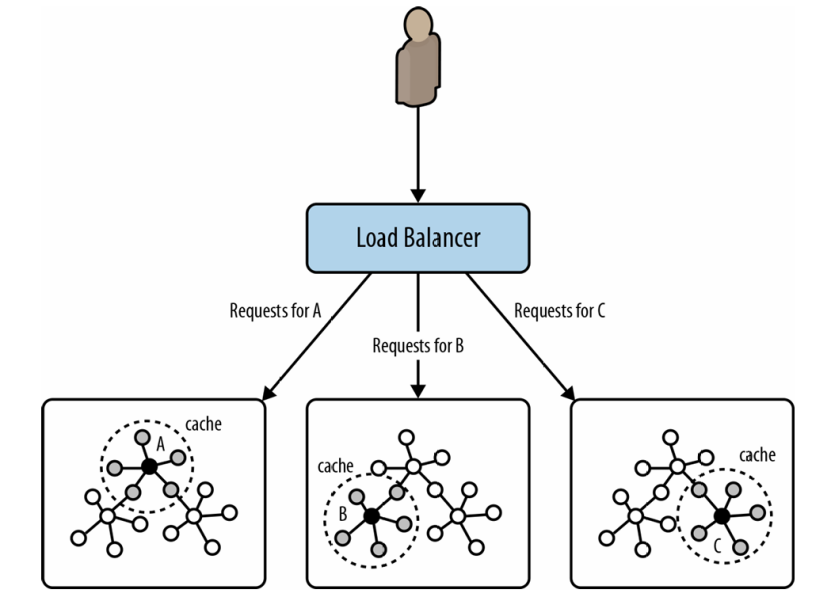
\includegraphics[width=0.8\textwidth]{images/26.png}
	\caption{分布式图存储}
	\label{fig:sharding}
\end{figure}

在TigerGraph中, 数据分片的方式通常基于节点的唯一标识符(例如节点的 ID), 系统会通过哈希函数将节点和边分配到不同的存储节点。这种方法保证了数据在集群中的均衡分布, 缓解了存储节点的负载不均衡问题。

此外, 分布式存储系统通常会实现多副本存储机制, 即每个数据分片在多个节点上都有副本。这些副本用于保证数据的高可用性和容错性。一旦某个节点出现故障, 其他节点上的副本可以继续提供数据访问服务, 从而保证系统的持续可用性。此外, 多副本机制也可以进行并行数据访问。

\subsubsection{分布式计算}
图数据的分布式计算框架通常采用迭代计算模型, 将复杂的图分析任务分解为多轮迭代执行的简单操作。在每轮迭代中, 计算任务被划分为映射(Map)和归约(Reduce)两个阶段。在映射阶段, 每个计算节点独立处理分配给它的图数据子集, 执行诸如节点值更新、边权重计算等局部操作。在归约阶段, 系统将各个节点的中间结果进行合并,完成全局计算。例如, 在计算社交网络的影响力分数时, 每个计算节点首先处理其负责的用户子集的直接关系网络, 然后通过多轮迭代逐步扩展影响范围, 最终汇总得到全局的影响力评分。为了提高计算效率, 框架会实现智能的任务调度策略, 根据数据分布和节点负载动态调整计算任务的分配。
\begin{figure}[H]
	\centering
	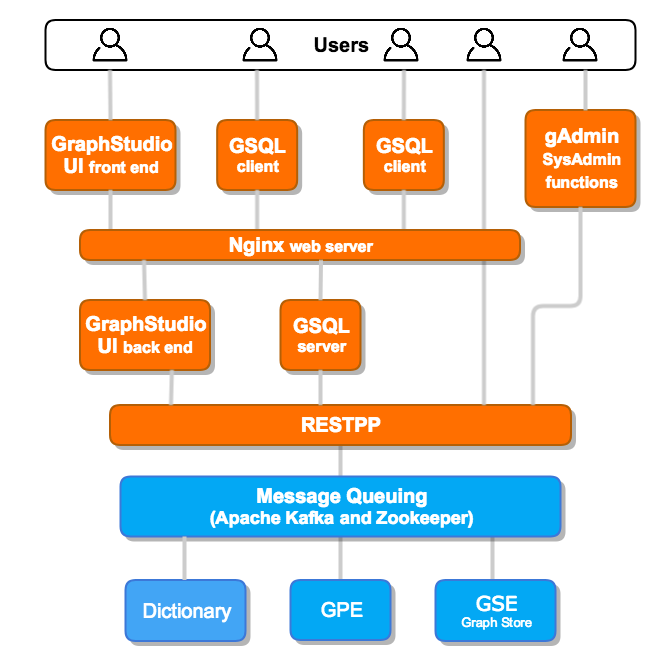
\includegraphics[width=0.6\textwidth]{images/25.png}
	\caption{TigerGraph的分布式计算架构}
	\label{fig:tigergraph}
\end{figure}
在TigerGraph中, GSQL查询在执行时会被分解为多个子任务, 这些子任务在不同的节点上并行执行, 充分利用了集群的计算能力。此外TigerGraph的分布式计算框架采用类似于Google Pregel的\textbf{超级步(Superstep)}模型。在超级步模型中, 每个节点都会在超级步中执行一系列计算任务, 然后与其他节点通信并同步。每个超级步的结果会影响下一步的计算, 直到所有节点完成计算为止。

最短路径查找: 当执行最短路径查找时, TigerGraph 会从源节点开始, 向外逐层遍历邻接节点。每个节点将其最短路径距离信息发送给其相邻节点, 直到找到目标节点。这种遍历过程是并行的, 并且多个节点可以同时处理不同的路径查找任务, 以加快查询速度。